% -------------------------------------------------------------------------------------------------
% Definitionen
% -------------------------------------------------------------------------------------------------
\documentclass[
    fontsize=12pt,                      % Schriftgröße 12 pt
    paper=a4,                           % Seitengröße A4
    twoside=off,                       % zweiseitiger Druck
    DIV=15,                             % Seiteneinteilung
    BCOR=12mm,                          % Bindekorrektur
    headings=normal,                    % normal große Überschriften
    headsepline=false,                   % Trennlinie unter der Kopfzeile
    footsepline=false,                  % Trennlinie über der Fußzeile
    headinclude=true,                   % Kopfzeile zählt zum Textkörper
    footinclude=false,                  % Fußzeile zählt nicht zum Textkörper
    toc=listof,                         % Verzeichnisse der Gleitumgebungen ins Inhaltsverzeichnis
    toc=bib,                            % Literaturverzeichnis ins Inhaltsverzeichnis
    chapterprefix=false,                % vor Kapitelnummern steht "Kapitel"
    appendixprefix=false,               % vor Anhangüberschriften steht "Anhang"
    numbers=noendperiod,                % Keinen Punkt hinter die letzte Zahl eines Kapitels (auch bei Anhang)
    captions=tableabove,                % Tabellenüberschriften setzen
    footnotes=multiple,                 % Erkennung von mehreren Fußnoten hintereinander
    bibliography=oldstyle,              % Literaturverzeichnis: openstyle oder oldstyle
    draft=false,                        % Entwurfsstadium
]{scrreprt}


% Paket Includes
% ----------------------------
\usepackage[T1]{fontenc}                % deutsche Umlaute und Sonderzeichen
\usepackage[utf8]{inputenc}             % Umlaute koennen direkt im Quelltext stehen
\usepackage[ngerman]{babel}             % neue deutsche Rechtschreibung 
\usepackage{lmodern}
\usepackage{graphicx}                   % Bilder einfügen
\usepackage{tabularx}                   % Tabellen mit fester Breite und variabler Spaltenbreite
\usepackage{array,longtable}            % Tabellen mit Seitenumbruch
\usepackage{booktabs}                   % bessere horizontale Linien in Tabellen
\usepackage{array,ragged2e}             % mehr Spaltentypen in Tabellen und neue Spaltentypen
\usepackage{dcolumn}                    % Spalten am Dezimaltrenner ausrichten
\usepackage{amsmath}
\usepackage[                            % Unterabbildungen mit folgenden Parametern:
            font=footnotesize,          % kleine Schrift
            labelfont={sf,bf},          % Labels fett und serifenlos
            textfont={sf},              % Text serifenlos
            format=hang,                % hängender Einzug
           ]{caption}
\usepackage{float}      
\usepackage{hyperref}                   % URL links     
\usepackage{xcolor}  
\usepackage{listings}

\definecolor{mygreen}{rgb}{0,0.6,0}
\definecolor{myred}{rgb}{0.7529,0.3137,0.3019}


\newcommand{\Farbcode}[1]{\texttt{\textbf{\textcolor{myred}{#1}}}}

% Kopf- und Fußzeile
% ----------------------------
\usepackage{scrlayer-scrpage} 
\setkomafont{pagehead}{\sffamily\small}
\setkomafont{pagefoot}{\sffamily\small}
%\automark{chapter}
\lohead{Modul Embedded Systems 2 -- Steuergeräte, Vernetzung, Software} \cohead{} \rohead{Übung 3-5}
\lofoot{\includegraphics[height=10pt]{Figures/HSMW-Logo-klein} HS Mittweida, INW, Prof. Thomanek}
\cofoot{} \rofoot{\thepage}

\pagestyle{headings}
\renewcommand*{\chapterpagestyle}{headings}% Nicht zu empfehlen, aber du willst das offenbar trotzdem.


\setcounter{secnumdepth} {3}
\addto\captionsngerman{\renewcommand{\figurename}{Abb.}}    % Verwende Abb. x.x anstatt Abbildung x.x
\renewcommand{\thefigure}{\arabic{figure}}
% -------------------------------------------------------------------------------------------------
% Dokument
% -------------------------------------------------------------------------------------------------

\begin{document}


\chapter*{Übung 3-5 -- Implementierung von Zustandsdiagrammen}

Implementieren Sie den Zustandsgraphen für die Verkehrs- und Fußgängerampel aus der Übung 3-4 von letzter Woche. 

\section*{1. Hardware-Aufbau}
Bauen Sie dafür zunächst die entsprechende Schaltung auf, bei der die Verkehrs- und Fußgängerampel per LEDs, der Signalknopf für die Fußgänger durch einen Taster und der Operator-Switch durch einen Schalter simuliert werden soll.
\noindent

\begin{figure}[H]
	\centering
	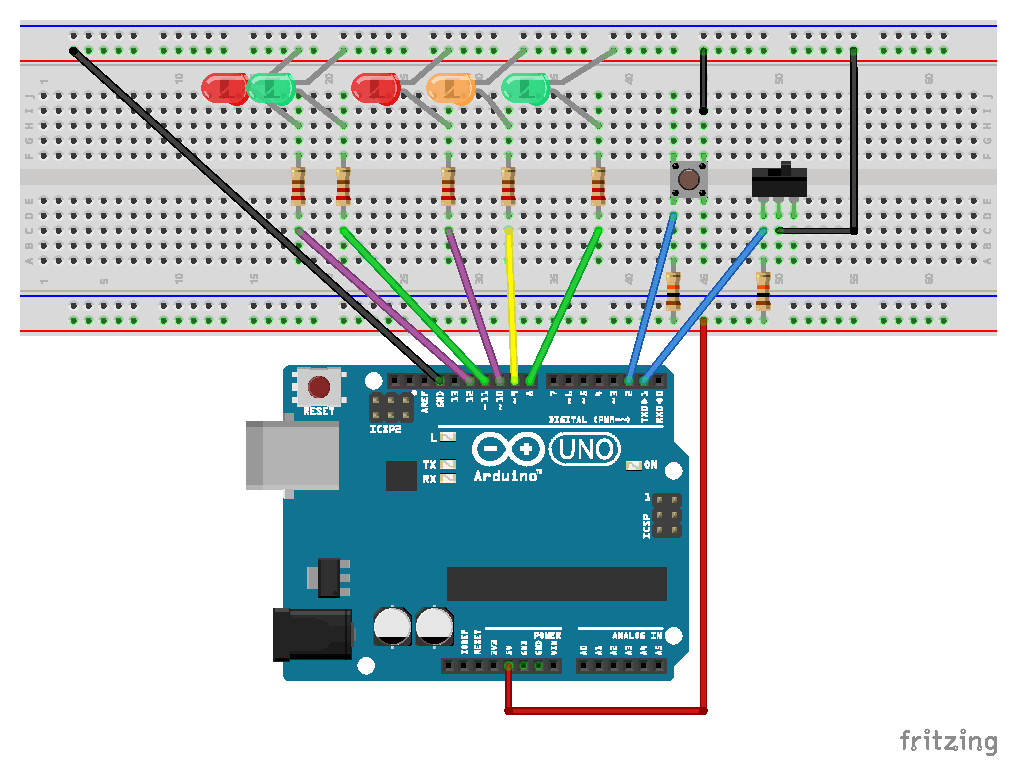
\includegraphics[width=\textwidth]{Figures/TrafficLight_Steckplatine}
\end{figure}

\section*{2. Zustandsautomat}
Als Grundlage für die Implementierung gilt folgender \textbf{Zustandsautomat}:
\begin{figure}[H]
	\centering
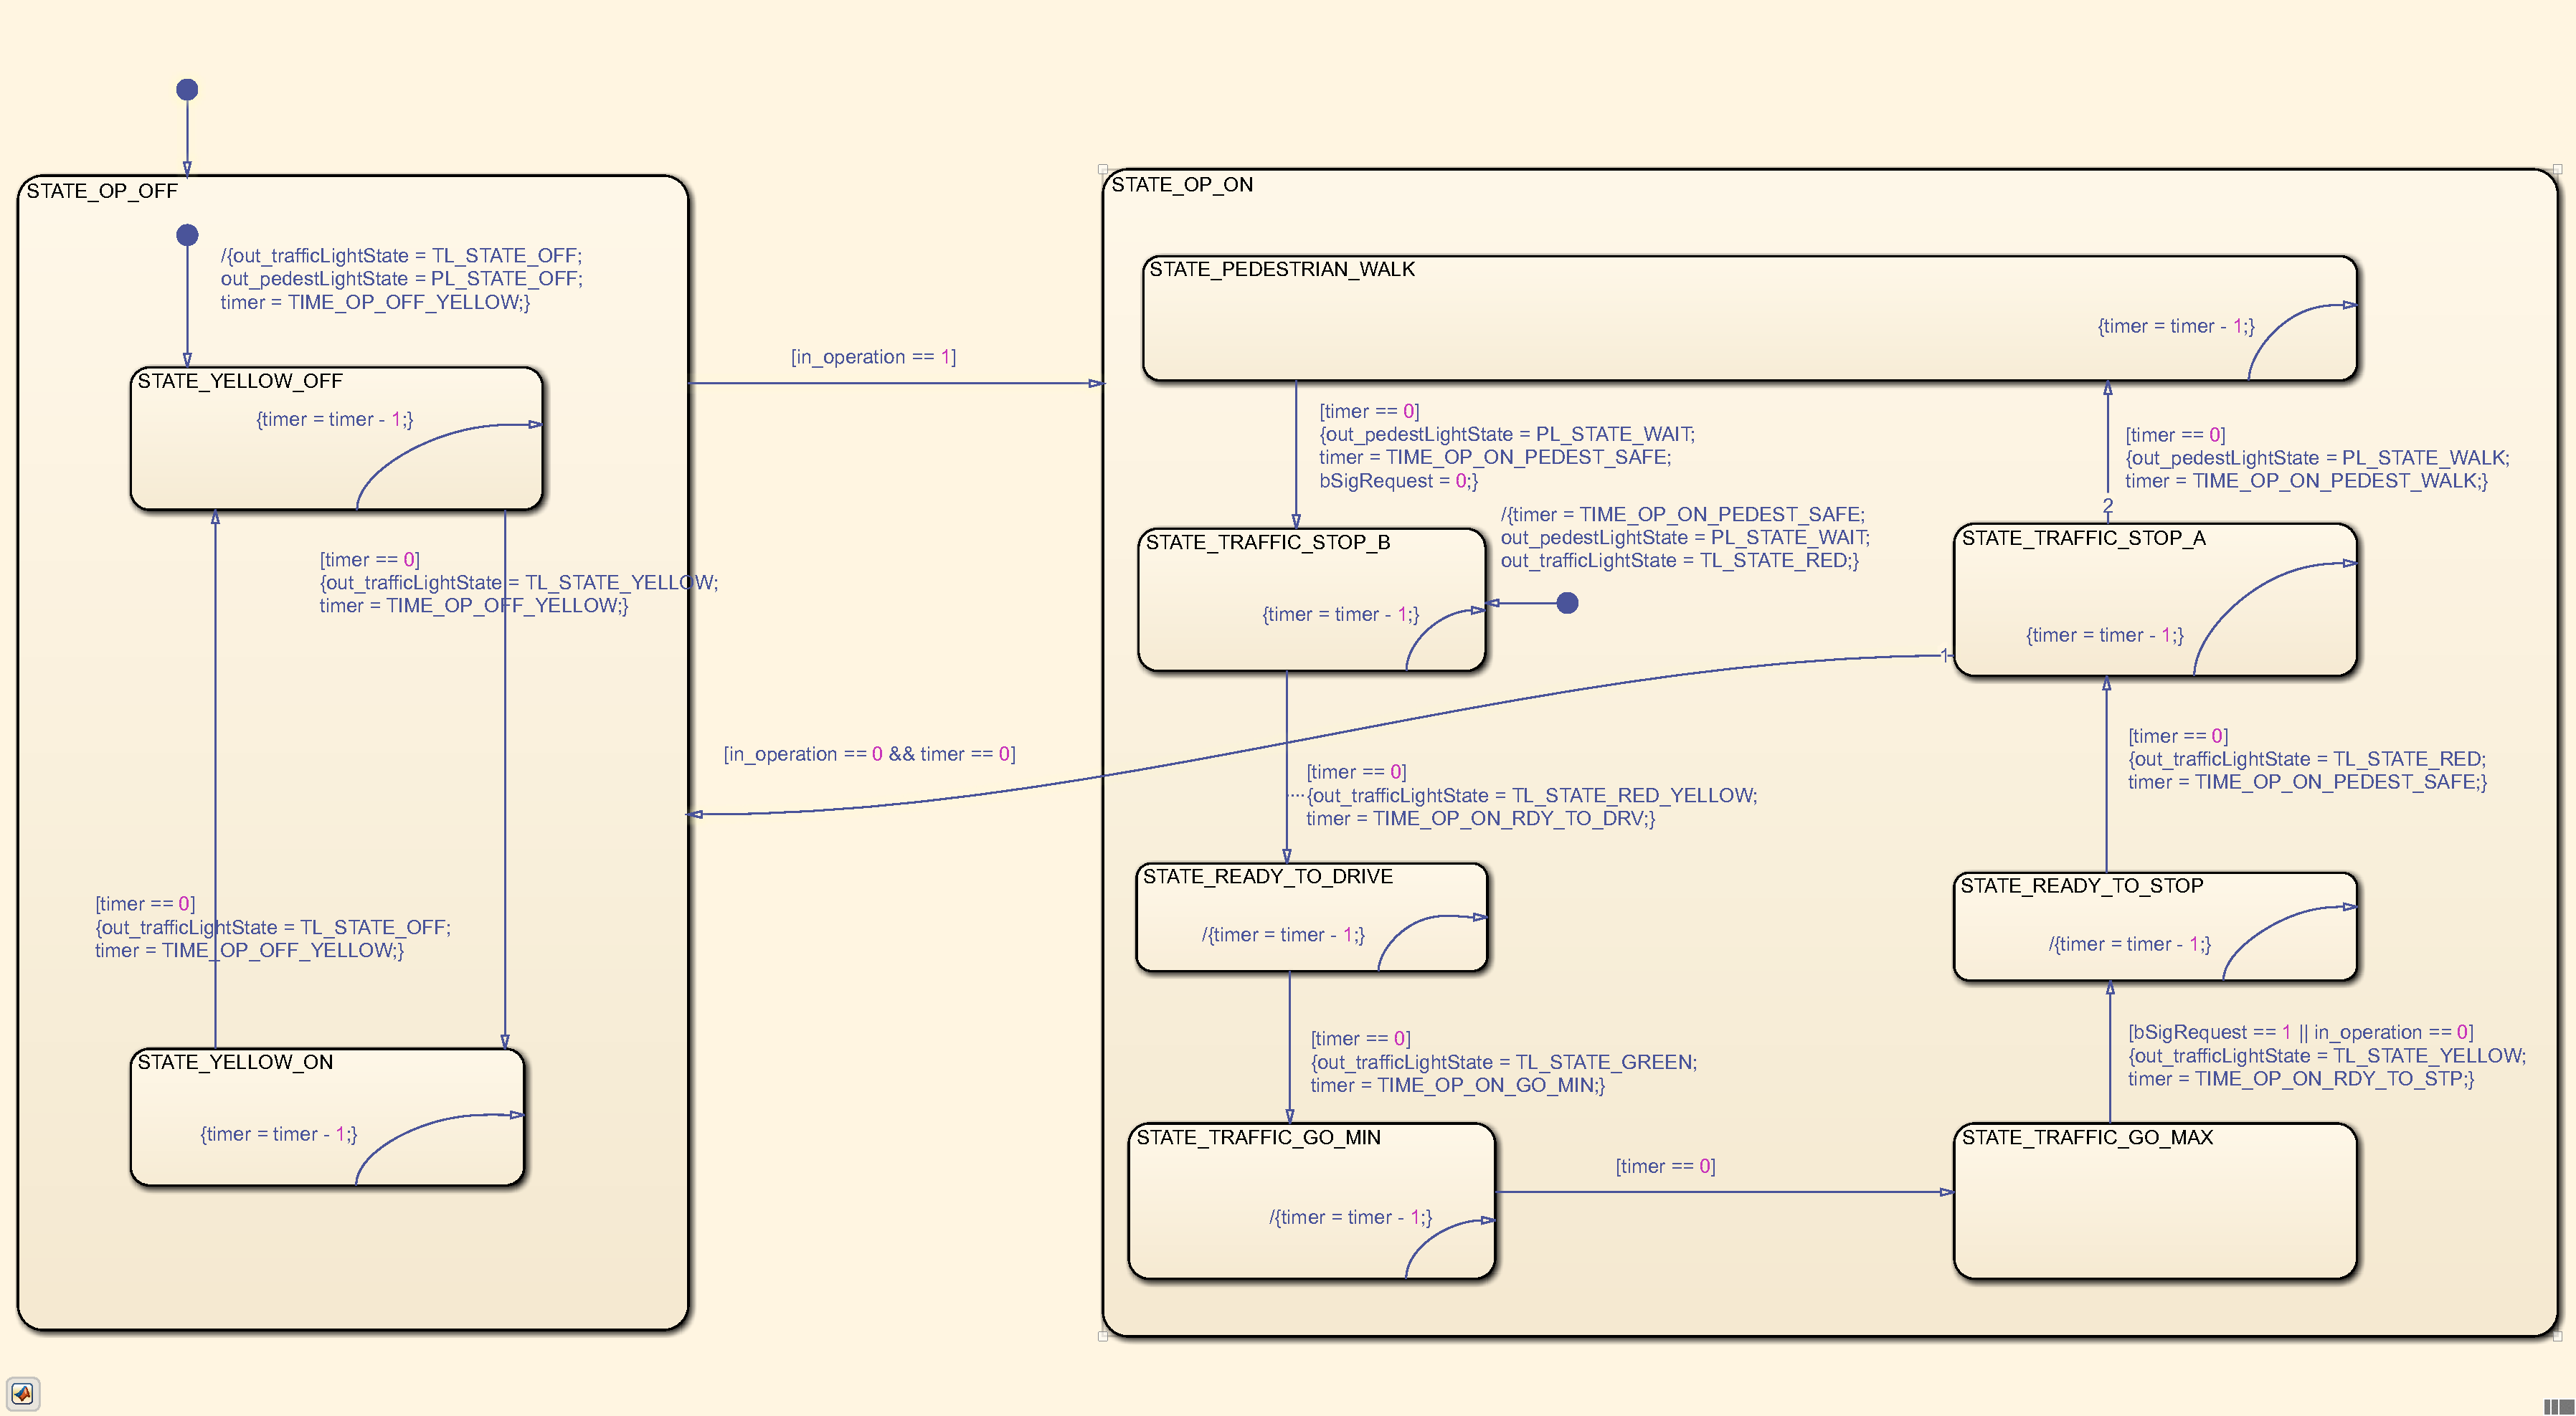
\includegraphics[width=\textwidth]{Figures/SM_TrafficLight_Traffic_Control}
\end{figure}

\section*{3. Objektorientierte Programmierung}
Das Softwareprojekt besteht aus den folgenden Dateien:
\begin{itemize}
	\item \Farbcode{CTrafficLight.h/CTrafficLight.cpp} -- Deklaration/Definition einer Klasse zur Kapselung der Verkehrsampel und deren Ansteuerung (\emph{siehe Klassendiagramm unten})
	\item \Farbcode{CPedesLight.h/CPedesLight.cpp} -- Deklaration/Definition einer Klasse zur Kapselung der Fußgängerampel und deren Ansteuerung (\emph{siehe Klassendiagramm unten})
	\item \Farbcode{CTrafficControl.h/CTrafficControl.cpp} -- Deklaration/Definition einer Klasse zur Steuerung der Verkehrs- und Fußgängerampel mittels einer Zustandsmaschine (\emph{siehe Klassendiagramm unten})
	\item \Farbcode{TrafficLight.ino} -- Arduino-Sketch zum Instanziieren der \Farbcode{CTrafficControl}-Klasse und zyklisches Aufrufen (aller 100~ms) deren Process-Methode zum Ausführen des Zustandsautomaten \\
	Des Weiteren zum Einlesen des Tasters und des Schalters
	
\end{itemize}
\begin{figure}[H]
	\centering
	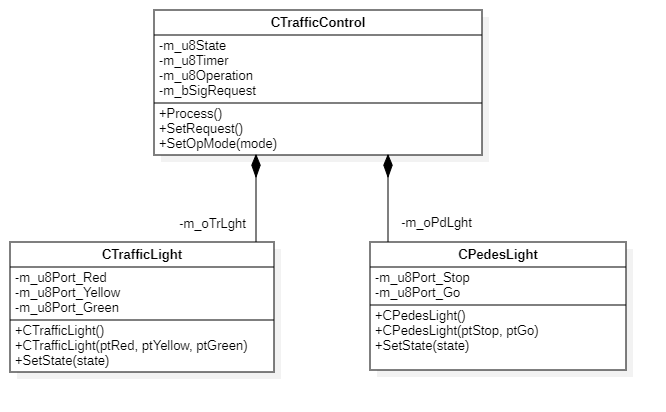
\includegraphics[width=\textwidth]{Figures/Klassendiagramm}
\end{figure}
\noindent
\textbf{Hinweise:}

\begin{itemize}
\item Im OPAL finden Sie diese Files bereits vorbereitet
\item Machen Sie sich mit den Klassen und ihren Inhalten vertraut
\item Im Wesentlichen besteht Ihre Aufgabe in der \textbf{Implementierung des Zustandsautomaten} in der Methode \Farbcode{Process()} der Klasse \Farbcode{CTrafficControl}
\item Um die Verkehrs- und Fußgängerampel zu schalten, rufen Sie aus der \Farbcode{Process()}-Funktion heraus jeweils die \Farbcode{SetState}()-Methode auf und übergeben als Parameter den gewünschten Zustand der Anzeige, wie bspw. \\ 
\Farbcode{SetState(CPedesLight::PL\_STATE\_WAIT)} oder \\
\Farbcode{SetState(CTrafficLight::TL\_STATE\_YELLOW)} 
\item [] (Die möglichen Anzeigezustände finden Sie als \Farbcode{enum}-Definition in der jeweiligen Header-Datei (\texttt{CTrafficLight.h},  \texttt{CPedesLight.h}))
\end{itemize}

 


\end{document}


